Alur, Madhusudan 2004 / Mehlhorn 1980 (input driven PDA)
\section{Motivation}
    \begin{itemize}
        \item Tradeoff: Ausdrucksstärke vs. Abschlusseigenschaften, Entscheidbarkeit
        \item guter Tradeoff: VPL
        \item PDA (Kellerautomat): Akzeptiert per leerem Keller
        \item DPDA (deterministischer Kellerautomat): Akzeptiert per Endzustand
        \item VPA ist eingeschränkter DPDA:
        \begin{itemize}
            \item Eingabezeichen bestimmen Kelleraktion
            \item Partitionierung des Alphabets:
            \subitem $\Sigma=\Sigmapush\dcup\Sigmapop\dcup\Sigmaneut$
            \subitem $\Sigmah=\left(Sigma_{push},\Sigmapop,\Sigmaneut\right)$
            \subitem push = call, pop = return, neutral = internal
        \end{itemize}
        \item Beispiel: $\Sigmah=\left(\{a\},\{b\},\{c\}\right)$
        \begin{itemize}
            \item $a^nb^n$
            \item $(a^nb^n)^*$
            \item $\{w\mid|w|_a=|w|_b\}\not\in VPL$
            \subitem $\rightarrow$ bei negativem Keller nie in VPL
        \end{itemize}
        \item Denkmodell: $\Delta w=|w|_{\Sigmapush}-|w|_{\Sigmapop}$
        \subitem $\rightarrow$ hat \qq{Zacken}, muss am Ende des Wortes wieder bei 0 sein
    \end{itemize}
\section{Definition: PDA}
    $M=(Q,Q_S,Q_F,\Gamma,\Sigmah,\delta,\#)$ mit:
    \begin{itemize}
        \item $Q$: Zustände
        \item $Q_S$: Startzustände
        \item $Q_F$: Endzustände
        \item $\Gamma$: Kelleralphabet
        \item $\hat\Sigma$: Eingabealphabet
        \item $\#$: Kellerbodenzeichen
        \item $\delta$: Übergänge
        \subitem $\delta \subseteq Q\times \Sigmaneut \times Q \\\cup Q\times \Sigmapush \times \Gamma\setminus\{\#\}\times Q\\\cup Q\times \Sigmapop \times\Gamma\times Q$
    \end{itemize}
\section{Semantik}
    \begin{itemize}
        \item Konfiguration: Element $Q\times\Sigmah^*\times \Gamma^*$
        \item Konfigurationsübergänge: Relation $\rightarrow \subseteq K\times K$
        \item $c\in\Sigmaneut:\ q,w_1,\dots,w_n,\gamma_1,\dots,\gamma_k\rightarrow \delta(q,c),w_1,\dots,w_{n-1},\gamma_1,\dots,\gamma_k$
        \item $a\in\Sigmapush:\ q,w_1,\dots,w_n,\gamma_1,\dots,\gamma_k\rightarrow q',w_1,\dots,w_{n-1},\gamma_1,\dots,\gamma_k,\gamma$
        \subitem $(q',\gamma)\in\delta(q,a)$
        \item $b\in\Sigmapop:\ q,w_1,\dots,w_n,\gamma_1,\dots,\gamma_k\rightarrow q',w_1,\dots,w_{n-1},\gamma_1,\dots,\gamma_{k-1}$
        \subitem $q'\in\delta(q,b,\gamma_k)$
        \item $L(M):=\left\{w\mid\exists s\in Q_S\exists f\in Q_F: s,w,\# \rightarrow^* f,\varepsilon,\# \text{ oder } \in\Gamma^*\#\right\}$
    \end{itemize}
\section{Alur-Kongruenz}
\subsection{Wiederholung: Myhill-Nerode}
    Myhill-Nerode-Relation in Abhängigkeit von $L\subseteq \Sigma^*$\\
    $u\sim_L v :\Leftrightarrow \forall x,y: xuy\in L \Leftrightarrow xvy\in L$ (syntaktische Kongruenz)\\
    $\Sigma^*/\sim_L=\{[w]|w\in\Sigma^*\}$ heißt syntaktisches Monoid
    \subsubsection{Anmerkungen}
        \begin{itemize}
            \item $[w_1][w_2]=[w_1w_2]$
            \item L regulär $\Leftrightarrow |\Sigma^*/\sim_L|$ endlich
        \end{itemize}
\subsection{Definition}
    $u,v\in WM$ (WM: Well-matched $\rightarrow$ akzeptieren mit leerem Keller im Endzustand)\\
    $u\simeq v :\Leftrightarrow \forall x,y\in\Sigma^*: xuy\in L\Leftrightarrow xvy\in L$
\subsection{Satz}
    $L$ ist VPL $\Leftrightarrow |WM/\simeq |$ endlich
\subsection{Anmerkungen}
    \begin{itemize}
        \item Operationen
            \begin{itemize}
                \item Konkatenation
                \item Extend:
                \subitem $[w]\rightarrow [awb],\ a\in\Sigmapush,b\in\Sigmapop$
            \end{itemize}
        \item $WM:=\{w\in\Sigma^* \mid \Delta(w)=0\wedge \forall i\le|w|:\Delta(w_1\dots w_i)\geq 0\}$
        \subitem mit $\Delta(w)=|w|_{\Sigmapush}-|w|_{\Sigmapop}$
        \item $\Sigma^* \supseteq L$ regulär $\rightarrow \Sigmah=(\emptyset,\emptyset,\Sigma)$
        \item Jedes visibly Wort lässt sich durch concat und extend erzeugen
    \end{itemize}
    \subsubsection{Beispiel}
    \vspace*{2cm}Leite $aaabbabb$ ab:\vspace*{-2.5cm}\\
        \hspace*{5cm}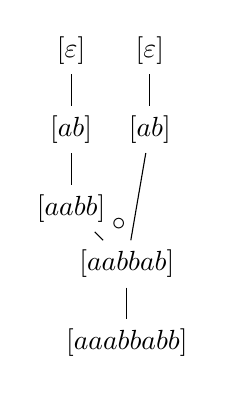
\begin{tikzpicture}
            \node (A) {$[\varepsilon]$};
            \node (Z) [right of=A] {$[\varepsilon]$};
            \node (B) [below of=A] {$[ab]$};
            \node (Y) [below of=Z] {$[ab]$};
            \node (C) [below of=B] {$[aabb]$};
            \node (D) [below right of=C] {$[aabbab]$}; \node[above of=D, yshift=-.5cm,xshift=-.1cm]{$\circ$};
            \node (E) [below of=D] {$[aaabbabb]$};
            \path (A) edge (B)
                (B) edge (C)
                (C) edge (D)
                (D) edge (E)
                (Z) edge (Y)
                (Y) edge (D);
        \end{tikzpicture}
\section{Satz}
    Für jeden VPA M existiert DVPA $M'$ mit L(M)=L($M'$) wobei L(M)$\subseteq$WM
    \subsubsection{Beweis}
    geg. $M=(Q,Q_S,Q_F,\Gamma,\Sigmah,\delta,\#)$, konstruiere $M'=(Q',q_S',Q_F',\Gamma',\Sigmah,\delta',\#)$
    \begin{itemize}
        \item $Q'=\mathcal{P}(Q\times Q)$
        \item $q_S'=\{(q,q)\mid q\in Q\}\in Q'$ (=$id_Q$)
        \item $Q_F'=\{S\in Q'\mid \exists s\in Q_S\exists f\in Q_F: (s,f)\in S\}$
        \item $\Gamma'=\Sigmapush\times Q'\cup \{\#\}$
        \item $\delta'$:
        \begin{itemize}
            \item $a\in\Sigmapush: \delta'(S,a)=(id_Q,(a,S))$
            \item $b\in\Sigmapop : \delta'(S,b,(a,S))=S''$\\%TODO: Formatting
            $S''=\{(q,q')\mid\exists q_1,q_2,q_3: (q,q_1)\in S', \exists\gamma\in\Gamma:(q_2,\gamma)\in\delta(q_1,a), (q_2,q_3)\in S, q'\in\delta(q_3,b,\gamma))\}$
            \item $c\in\Sigmaneut: \delta'(S,c)=\{(q,q')\mid \exists q''\in Q: (q,q'')\in S\wedge q'\in \delta(q'',c)\}$
        \end{itemize}
    \end{itemize}
\section{Satz von Chomsky-Schützenberger, 1963}
    Jede kontextfreie Sprache ist das homomorphe Bild einer Sprache $\mathds{D}_{2k}\cap R$ wobei $R$ regulär.\\
    $\forall L\subseteq \Sigma^*\text{ kf. }\exists k\in\mathds{N}, R\text{ reg. }\exists\varphi:L=\varphi(\mathds{D}_{2k}\cap R)$ $\varphi:\Sigma^*\rightarrow \{[_1,]_1,[_2,]_2,\dots\}^*$
    \subsection{Beweis}
        $L$ kf $\Rightarrow\exists G=(V,\Sigma,P,s)$ mit $L(G)=L$ und $L$ in CNF\\
        $X\in L(G)\Leftrightarrow\exists$ Ableitungsbaum (mit CNF: Binärbaum)\\
        Idee: Nutze Korrespondenz zwischen Bäumen und Dyck-Sprachen.\\\vspace{2mm}
        Konstruiere Grammatik $G'=(V',\Sigma',P',S')$ wobei $L(G')=\mathds{D}_{2k}\cap R$\\
        Sei $P=\{\Pi_1,\dots,\Pi_k\}$, dann $P'=\{\Pi_1',\dots,\Pi_k'\}$
        \begin{itemize}
            \item ist $\Pi_i=A\rightarrow BC$, dann $\Pi_i'=A\rightarrow\mathop{[}\limits_i^1B\mathop{]}\limits_i^1\mathop{[}\limits_i^2C\mathop{]}\limits_i^2$
            \item ist $\Pi_i=A\rightarrow a$, dann $\Pi_i'=A\rightarrow\mathop{[}\limits_i^1\mathop{]}\limits_i^1\mathop{[}\limits_i^2\mathop{]}\limits_i^2$
        \end{itemize}
        $\Sigma'=\{\mathop{[}\limits_i^1,\mathop{]}\limits_i^1,\mathop{[}\limits_i^2,\mathop{]}\limits_i^2,\dots,\mathop{[}\limits_k^1,\mathop{]}\limits_k^1,\mathop{[}\limits_k^2,\mathop{]}\limits_k^2\}$\\
        Wähle $\varphi:\Sigma'\rightarrow\Sigma$:
        \begin{itemize}
            \item Ist $\Pi_i=A\rightarrow BC$, so $\varphi(\mathop{[}\limits_i^1)=\varphi(\mathop{]}\limits_i^1)=\varphi(\mathop{[}\limits_i^2)=\varphi(\mathop{]}\limits_i^2)=\varepsilon$
            \item Ist $\Pi_i=A\rightarrow a$, so $\varphi(\mathop{]}\limits_i^1)=\varphi(\mathop{[}\limits_i^2)=\varphi(\mathop{]}\limits_i^2)=\varepsilon,\varphi(\mathop{[}\limits_i^1)=a$
        \end{itemize}
        \begin{enumerate}[1)]
            \item $L=\varphi(L(G'))$
            \item $L(G')=\mathds{D}_{2k}\cap R$
        \end{enumerate}
        \begin{enumerate}[1)]
            \item $x\in L \Leftrightarrow x\in L(G)\\\Leftrightarrow \exists$ Ableitungsbaum von G für $x\\\Leftrightarrow x'\in L(G'),$ wobei $x'$ Klammerrepräsentation des Baumes ist$\\\Leftrightarrow x\in\varphi(L(G'))$, da für jedes Blatt das richtige Zeichen übrig bleibt
            \item offensichtlich: $L(G')\subseteq\mathds{D}_{2k}$\\
            Weitere Bedingungen an die Wörter, um Konstruktion zu genügen:
            \begin{enumerate}[a)]
                \item einem $\mathop{]}\limits_i^1$ muss immer $\mathop{[}\limits_i^2$ folgen
                \item einem $\mathop{]}\limits_i^2$ muss $\mathop{]}\limits_j^1$ oder $\mathop{]}\limits_j^2$ folgen (beachte Sonderfall für Startvariable)
                \item ist $\Pi_i=A\rightarrow BC$, dann muss $\mathop{[}\limits_i^1$ ein $\mathop{[}\limits_p^1$ folgen mit $\Pi_p=B\rightarrow EF$ oder $\Pi_p=B\rightarrow b$ und $\mathop{[}\limits_i^2$ muss immer $\mathop{[}\limits_q^1$ folgen mit $\Pi_q=C\rightarrow GH$ oder $\Pi_q=C\rightarrow c$
                \item ist $\Pi_i=A\rightarrow a$, dann muss auf $\mathop{[}\limits_i^1$ $\mathop{]}\limits_i^1$ folgen und auf $\mathop{[}\limits_i^2$ $\mathop{]}\limits_i^2$ und auf $\mathop{]}\limits_i^1$ $\mathop{[}\limits_i^2$
                \item $\mathop{[}\limits_i^1$ als erstes Zeichen, dann muss $\Pi_i$ S auf der linken Seite haben
            \end{enumerate}
            \item[$\rightarrow$] Bedingungen sind alle regulär. Schneide alle Sprachen dieser Bedingungen; erhalte $R$, regulär.
        \end{enumerate}
